\section{Anpassung der existierenden Lösung}
Infrastrukturelle Anpassungen wurden im Buildsystem vorgenommen. Herausfordernd war das initiale Setup des bestehenden
Projekts, da hierfür die Installation von externen Abhängigkeiten notwendig ist. Außerdem müssen Dateistrukturänderugen
in der Builddatei von CMAKE reflektiert werden. Um die zukünftige Installation auf weiteren Systemen zu vereinfachen,
wurde das Buildtool CMAKE angepasst und das Projekt zur Befehlsaggregation mit einer Makefile ergänzt.


\subsection{CMAKE}
\label{sec:cmake}
Absolute Pfadreferenzen in der bestehenden Implementierung erschwerten die gemeinsame Arbeit und den Build an einer
Codebasis, weswegen die CMAKE-Files und die Struktur des Codes angepasst wurde. Um das Setup des Projekts zu
vereinfachen wurde der Paketmanager VCPKG als GIT-Submodule zum Repository hinzugefügt. Mit dem Clone des Repositories
wird dann auch der Paketmanager installiert, welcher die Referenzierung von Abhängigkeiten mit relativen Pfaden
ermöglicht. Durch das verwenden des VCPKG package manager können die Abhängigkeiten durch die CMAKE-Befehle
\textit{find\_package} und \textit{find\_path} eingebunden werden. Eine manuelle Anpassung der Pfade ist dann nicht mehr
notwendig.\\


\subsection{Makefile}
Eine definierte Makefile bietet die Möglichkeit zur Ausführung von Befehlssequenzen über einfache Aggregatsbefehle.
So kann der Paketmanager selbst und alle eingebundenen Abhängigkeiten mit zwei Befehlen installiert werden.
Die Kompilierung des Projektes ist ebenfalls mit einem Makebefehl möglich, sodass vorher nötige manuelle Anpassungen nun
osolet sind. Dies ist in Listing \ref{code:Makefile} dargestellt.\\

\begin{lstlisting}[caption=Makefile, label={code:Makefile}, captionpos=b]
    .PHONY: about init install-dependencies build compile start-subscale start-server start-client kill-server clean

    VCPKG_DIR := ./include/vcpkg
    VCPKG := ./include/vcpkg/vcpkg
    
    about:
	    @echo "Makefile to help manage subscale gpu project"
	    @echo "commands:"
	    @echo "     - init: make sure vcpkg ist cloned as submodule"
	    @echo "     - install-dependencies: install all vcpkg dependencies"
	    @echo "     - build: build cmake changes"
	    @echo "     - compile: compile the code"
	    @echo "     - start-subscale: start subscale local"
	    @echo "     - start-server: starts a server to which the client sends data to   calculate"
	    @echo "                     default port is 8080, else set with     -p=<port-number>"
	    @echo "     - start-client: starts execution subscale distributed"
	    @echo "     - kill-server: kills all servers still running in background"
	    @echo "     - removes builded files"
    
    init:
        git submodule update --init --recursive && $(VCPKG_DIR)/bootstrap-vcpkg.sh && mkdir Proto/generated
    
    install-dependencies:
        $(VCPKG) install nlohmann-json && $(VCPKG) install mlpack && $(VCPKG) install grpc
    
    build:
        cmake -S . -B ./debug
    
    compile:
        cmake --build ./debug
    
    start-subscale:
        ./debug/Subscale/subscale
    
    start-server:
        ./debug/Server/server $(p)
    
    start-client:
        ./debug/Client/client
    
    kill-server:
        killall ./debug/Server/server
    
    clean:
        rm -rf ./debug
\end{lstlisting}

Durch die Verwendung dieser Makefile-Befehle soll es vereinfacht werden, den Code zum einen manuell in seiner eignen
Umgebung ausführen zu können, als auch zum anderen automatisiert innerhalb eines Docker-Containers.

Da das \verb|vcpkg| als Submodule integriert wurde, was die automatisierte Installation und Pfadfindung von \verb|vcpkg|
als auch \verb|gRPC|, \verb|mlpack| und \verb|nlohmann-json| ermöglicht, können alle benötigten Schritte per
\verb|make init| (Zeilen 20f) und \verb|make install-dependencies| (Zeilen 23f) sehr einfach und automatisiert
installiert und integriert werden. Es besteht weiterhin die Möglichkeit die CMakeLists-Files manuell anzupassen und
diese beiden Makefile-Befehle zu ignorieren. Dies ist sinnvoll, wenn man Docker-Container besitzt, welche dies im
Vorhinein bereits installiert haben oder das \verb|vckpg| aus der eigenen Entwicklungsumgebung genutzt werden soll.

Der Build des Projekts mit CMAKE wird über den Befehl \verb|make build| (Zeilen 26f) abgestoßen. Mit \verb|make compile|
(Zeilen 29f) ist die Kompilierung möglich.

\verb|make start-subscale| (Zeilen 32f) führt den Subscale-Algorithmus lokal aus. \verb|make start-server| (Zeilen 35f)
beziehungsweise \verb|make start-client| (Zeilen 38f) startet Server und Client bei einer gewünschten verteilten
Ausführung. Das Serverkommando bietet außerdem die Möglichkeit zur Übergabe eines Ports, auf welchem der Server lauschen
soll. \verb|make start-server -p=8080| startet einen Server, welcher über den Port 8080 erreichbar ist.

\verb|make kill-server| beendet alle im Hintergrund laufenden Server über deren Prozess-ID.

\verb|make clean| (Zeilen 44f) bereinigt die Maschine von allen gebauten Projektdaten.

\subsection{Umstrukturierung}
Beim gegebenen Code handelte es sich um ein Ein-Mann-Projekt. Damit im Team unabhängig und konfliktfrei gearbeitet
werden kann, muss die Codebasis umstrukturiert werden. Der gegebene Code clusterte sich wie folgt:
\dirtree{%
.1 data.
.1 packages.
.1 SubscaleGPU.
.2 ....
.1 CMakeLists.txt.
.1 config.json.
}
Die Logik für den gesamten Subscale-Algorithmus befand sich im Ordner \textit{SubscaleGPU}. Die zugehörigen Daten im
\textit{data} Ordner. Zusätzlich benötigte Libraries befanden sich im \textit{packages} Ordner. Die Aktuelle Struktur
erschwerte die Umwandlung in eine Client-Server-Architektur. Der Code muss umstrukturiert werden, damit gleichzeitig an
Client, Server und dem Subscale-Algorithmus gearbeitet werden kann. Der gesamte Subscale Algorithmus wurde in einen
eigenen Ordner verschoben und als statische Library weiterentwickelt. Somit kann dieser im Client und Server
eingebunden werden. Des Weiteren benötigen sowohl Client als auch Server die Protobuf-Dateien. Für diese wurde ebenfalls
ein eigener Ordner angelegt. Sowohl Client, als auch Server konsumierten die Schnittstellendefinitionsdateien um daraus
Skeletons und Stubs zu generieren.
Die neue Struktur gliederte sich wie folgt:

\dirtree{%
.1 Client.
.1 include.
.2 vcpkg.
.1 Proto.
.2 subscale.proto.
.1 Server.
.1 SubscaleGPU.
.2 data.
.2 Config.
.1 CMakeLists.txt.
}

\subsection{Aufbau der gegebenen Implementierung}
Die gegebene Implementierung enthält die Klasse \emph{LocalSubspaceTable}, welche die \emph{Subspace}-Tabelle darstellt.
Diese Klasse wurde sowohl für die Berechnung der \emph{Slices}, als auch für die Berechnung ganzer \emph{Subspaces}
verwendet. Folglich wurde die Logik mit einer Funktion \emph{calculateRemote} abstrahiert, die als Parameter
\emph{Labels}, sowie die \emph{min-} und \emph{maxBound} eines Slices erhält, um daraus Einträge für den
\emph{LocalSubspaceTable} zu generieren.

Im Folgenden wird zunächst der Aufbau der gegebenen Implementierung erläutert, um anschließend die Umsetzung der
\emph{calculateRemote}-Methode zu demonstrieren..\\
Der Code bestand im wesentlichen aus einer abstrakten Klasse \emph{ISubscale} und zwei konkreten Implementierungen
\emph{Subscale} (\emph{Cuda}-Implementierung) und \emph{SubscaleSec} (sequenzielle Implementierung) wie im folgenden
gezeigt:
\newpage
\begin{figure}[h]
    \centering
    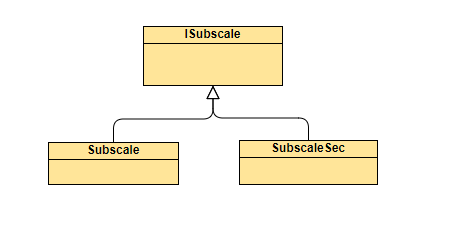
\includegraphics[width=\textwidth]{Subscale.png}
    \caption{Subscale}
    \label{img:subscale}
\end{figure}

\emph{ISubscale} implementiert die Funktion \emph{calculateClusterCandidates} welche generische vorbereitende Maßnahmen
für eine konkrete Subscale Implementierung trifft. Die Ausführung des eigentlichen Algorithmus geschieht mit der
abstrakten Methode \emph{calculateAllSlices}. Diese Methode berechnet alle Slices, je nach eingebundener Implementierung
entweder sequenziell oder parallel auf der Grafikkarte, und schreibt die Ergebnisse auf die Festplatte. Die abstrakte
Methode \emph{combineAllSlices} kombiniert alle im vorherigen Schritt berechneten Slices zu einer Tabelle mit möglichen
Clusterkandidaten.

\subsection{calculateSlice}
In einer neuen Funktion wird die Erstellung der Slices abstrahiert. Diese Funktion erhält alle nötigen Informationen
zur Berechnung eines Slices. Die folgende Sektion behandelt die generischen Funktionalitäten der Funktion. Unterschiede
der konkreten Implementierung in Ableitungen werden im Anschluss erläutert.

\lstinputlisting[language=C++,caption={calculateSlice},
    label=lst:calculateSlice]{src/calculateSlice.cpp}

Wie in Listing \ref{lst:calculateSlice} zu sehen ist, werden die Berechungsklassen initialisiert und anschließend
\emph{DenseUnits} erzeugt, um diese einer Subspace Tabelle hinzuzufügen. Sollte der \emph{Slice} nicht leer sein,
werden die Einträge anhand der Subspaces zusammengefügt. Schlussendlich wird der Speicher der Grafikkarte zum Host
kopiert (ist bei der sequentiellen Abarbeitung nicht nötig).

\subsection{calculateSlice Sequentiell}
In dieser Sektion werden die spezifischen Erzeugungen der Berechungsklassen für die sequenzielle Abarbeitung gezeigt.

\lstinputlisting[language=C++,caption={calculateSlice Sequentiell},
    label=lst:calculateSliceSeq]{src/calculateSliceSeq.cpp}

\subsection{calculateSlice Cuda}
In dieser Sektion werden die spezifischen Erzeugungen der Berechungsklassen für die \emph{Cuda} Abarbeitung gezeigt.

\lstinputlisting[language=C++,caption={calculateSlice Cuda},
    label=lst:calculateSliceCuda]{src/calculateSliceCuda.cpp}

\subsection{calculateClusterCandidatesRemote}
Ein vorheriger Schritt, die \emph{calculateClusterCandidatesRemote}-Methode, bereitet alle notwendigen
Informationen für die \emph{calculateSlice} vor. Diese Methode sieht wie folgt aus:

\lstinputlisting[language=C++,caption={calculateClusterCandidatesRemote},
    label=lst:calculateClusterCandidatesRemote]{src/calculateClusterCandidatesRemote.cpp}

Diese hat die \emph{CoreSets} erzeugt und die weiteren Informationen in den nächsten Schritt gegeben.

\subsection{calculateRemote}
Die \emph{calculateRemote}-Methode, ließt schlussendlich die \emph{config} und erzeugt die konkrete Implementierung
des \emph{Subscales}.

\lstinputlisting[language=C++,caption={calculateRemote},
    label=lst:calculateRemote]{src/calculateRemote.cpp}
